\documentclass{article}
\usepackage{amssymb}
\usepackage{amsmath}
\usepackage{enumitem}
\usepackage{tikz}
\usetikzlibrary{arrows.meta, calc}


\begin{document}

  \section{Punto 1)}
      Demuestre que $D_n = \mathbb{Z}_2 \Join \mathbb{Z}_n$ encontrando el isomorfismo 
      $\phi$ correcto. Deduzca que el producto semidirecto de grupos abelianos no es abeliano.

      Vamos a deducir qué propiedades debería de cumplir $\phi$ para concluir el 
      isomorfismo entre $D_n$ y el producto semidirecto.

      Si es un homomorfismo, se debe seguir inmediatamente que $\phi(0) = I_{\mathbb{Z}_n}$ y 
      de la propiedad 2 enunciada, se debe seguir que $h k h^{-1} = \phi(h)(k)$. 

      Como los únicos elementos de $\mathbb{Z}_2$ son $0, 1$ y ya tenemos el valor de 
      $\phi$ en $0$, entonces la propiedad enunciada arriba se debe seguir para para 
      $1$, pero como queremos un isomorfismo con $D_n$, entonces podríamos decir que 
      $1$ sería el equivalente a la reflexión. 

      Así mismo, el $1'$ de $\mathbb{Z}_n$ sería el equivalente a la rotación de $D_n$. En 
      términos de parejas ordenadas, $s \sim (1, 0)$ y $r \sim (0, 1)$. 

      Como sabemos que $s r^j s = r^{-j}$, entonces se define
      \begin{equation*}
        \begin{aligned}
          \phi(1): \mathbb{Z}_n &\to \mathbb{Z}_n \\
          k &\mapsto n - k 
        \end{aligned}
      \end{equation*}

      Básicamente, es el isomorfismo que toma un elemento y lo envía a su inverso.

      Debemos verificar que $\phi$ sea un homomorfismo, es decir, que $\phi(x + y) = \phi(x) \circ \phi(y)$.

      \begin{enumerate}[label=(\alph*)]
        \item Si $x \neq y$: Entonces alguno de los dos es el $0$ de $\mathbb{Z}_2$, luego, 
              $\phi(x + y) = \phi(y)$ o $\phi(x + y) = \phi(x)$, en cualquier caso, se cumple,
              pues el contrario sería la función identidad y se concluiría que 
              $\phi(x + y) = \phi(x) \circ \phi(y)$.

        \item Si $x = y$, entonces $x + y = 0$. Si $x = 0$, es inmediato. Si $x = 1$, entonces 
              bastaría probar que $\phi(1) \circ \phi(1) = I_{\mathbb{Z}_n}$. 
              $(\phi(1) \circ \phi(1)) (k) = \phi(1)(\phi(1)(k)) = \phi(1)(n-k) = k$, concluyendo así que 
              $\phi(x + y) = \phi(x) \circ \phi(y)$.
      \end{enumerate}

      Con todo esto, vamos a ver ahora si que $D_n \equiv \mathbb{Z}_2 \Join \mathbb{Z}_n$.

      Definimos la siguiente función:
      \begin{equation*}
        \begin{aligned}
          \Psi: D_n &\to \mathbb{Z}_2 \Join \mathbb{Z}_n \\
          s^i \cdot r^j &\mapsto (i, \phi(i)(j))
        \end{aligned}
      \end{equation*}

      Verifiquemos que $\Psi$ es un homomorfismo, es decir, que 
      $\Psi(s^i r^j \cdot s^k r^l) = \Psi(s^i r^j) \cdot \Psi(s^k r^l)$.

      Primero, usamos la relación $sr^j s = r^{-j}$ para simplificar el producto en $D_n$:
      \[
        s^i r^j \cdot s^k r^l = s^{i+k} \cdot r^{(-1)^k j + l}
      \]
      pues si $k = 0$ es inmediato, y si $k = 1$, entonces 
      $s^i r^j \cdot s r^l = s^i \cdot (r^j s) \cdot r^l = s^i \cdot s r^{-j} \cdot r^l = s^{i+1} r^{l - j}$.

      Entonces, aplicando $\Psi$:
      \[
        \Psi(s^i r^j \cdot s^k r^l) = \left(i + k,\; \phi(i+k)\!\left((-1)^k j + l\right)\right)
      \]

      Por otro lado, usando la operación del producto semidirecto:
      \[
        \begin{aligned}
          \Psi(s^i r^j) \cdot \Psi(s^k r^l) 
          &= (i,\, \phi(i)(j)) \cdot (k,\, \phi(k)(l)) \\
          &= \left(i + k,\; \phi(i)(j) + \phi(i)(\phi(k)(l))\right) \\
          &= \left(i + k,\; \phi(i)\!\left(j + \phi(k)(l)\right)\right)
        \end{aligned}
      \]
      donde en el último paso usamos que $\phi(i)$ es un homomorfismo de $\mathbb{Z}_n$.

      Debemos verificar que ambas expresiones coinciden, es decir, que 
      $\phi(i)(j + \phi(k)(l)) = \phi(i+k)((-1)^k j + l)$.
      Analizamos los cuatro casos posibles en $\mathbb{Z}_2$:

      \begin{enumerate}[label=(\alph*)]
        \item $i = 0, k = 0$: Ambos lados dan $j + l$.
        \item $i = 0, k = 1$: El lado izquierdo es $j + \phi(1)(l) = j + (n - l)$, y el derecho es 
              $\phi(1)(l - j) = n - (l - j) = j + (n - l)$.
        \item $i = 1, k = 0$: Ambos lados dan $\phi(1)(j + l) = n - j - l$. 
        \item $i = 1, k = 1$: El lado izquierdo es $\phi(1)(j + \phi(1)(l)) = \phi(1)(j + n - l) = n - (j + n - l) = l - j$, 
              y el derecho es $\phi(0)(l - j) = l - j$.
      \end{enumerate}

      Luego, $\Psi$ es un homomorfismo. Es sobreyectivo pues cualquier pareja ordenada $(i, k)$ 
      tiene pre-imagen $s^i r^{(\phi(i)^{-1}(k))}$, ya que 
      $\Psi(s^i r^{\phi(i)^{-1}(k)}) = (i, \phi(i)(\phi(i)^{-1}(k))) = (i, k)$.

      Ahora, si $\Psi(s^i r^j) = (0, 0)$, entonces $(i, \phi(i)(j)) = (0, 0)$, luego $i = 0$, y 
      entonces $j = \phi(0)(j) = 0$, así que $\Psi$ es inyectivo. Por lo tanto, es un isomorfismo.

      Finalmente, sabemos que tanto $\mathbb{Z}_2$ y $\mathbb{Z}_n$ son grupos abelianos, pero $D_n$ no 
      es un grupo abeliano, concluyendo así que el producto semidirecto de grupos abelianos no es, necesariamente, 
      abeliano.

  \section{Punto 2)}
    Sean $p$ y $q$ dos primos con $p < q$ y $p|(q - 1)$. Demuestre que, a menos de isomorfismos, hay solo dos 
    grupos de orden $pq: \mathbb{Z}_p \times \mathbb{Z}_q$ y $\mathbb{Z}_p \Join \mathbb{Z}_q$.

    Llamemos $G$ el grupo de orden $pq$ que cumple las demás condiciones.
    Usando el teorema de Sylow, sabemos que existen subgrupos de orden $p$ y de orden $q$. Por este teorema 
    también sabemos que $n_p$, la cantidad de subgrupos de orden $p$ cumple que 

    \begin{equation*}
      \begin{aligned}
        n_p \equiv 1 &\mod p \\
        n_p &| q
      \end{aligned}
    \end{equation*}

    Similarmente para $n_q$:

    \begin{equation*}
      \begin{aligned}
        n_q \equiv 1 &\mod q \\
        n_q &| p
      \end{aligned}
    \end{equation*}

    Como $n_q | p$, entonces $n_q = 1 \lor\, n_q = p$. Sabemos que 
    $n_q = 1, 1 + q, 1 + 2q, ...$ entonces $p$ debería ser alguno de esos valores, si no es $1$
    se contradice, pues cualquiera de los otros valores haría que $p > q$ pero se está asumiendo 
    lo contrario; entonces, $n_q = 1$, por lo tanto, solo hay un subgrupo de orden $q$ y por 
    consecuencias del teorema de Sylow, este grupo es normal en $G$.

    Ahora, para hallar un valor para $n_p$, sabemos que $n_p | q$, luego, $n_p = 1 \,\lor\, n_p = q$, 
    pero como $n_p = 1, 1 + p, 1 + 2p, ...$ entonces $n_p = 1 \,\lor\, n_p = 1 + kp$, donde 
    $kp = q - 1$.

    Entonces tenemos asegurada la existencia de un subgrupo $H$ de orden $p$ y de un 
    subgrupo $K$ de orden $q$, con $K \trianglelefteq G$. Supongamos que $n_p = 1$ y 
    tomemos el homomorfismo trivial 
    entre $H$ y Aut$(K)$, entonces el producto semidirecto $H \Join K$ es $H \times K$. 
    Vamos a demostrar que esto define un isomorfismo con $G$.

    Como $H \cap K = \{e\}$ y ambos son normales (sumimos que $n_p = 1$). Sean 
    $h \in H$ y $k \in K$. Demostraremos que $hk = kh$ (equivalente a mostrar que $hkh^{-1}k^{-1} = e$).


    Como $hkh^{-1} \in K$, por ser $K$ normal, entonces $hkh^{-1}k^{-1} \in K$, similarmente, 
    $kh^{-1}k^{-1} \in H$ y por lo tanto $hkh^{-1}k^{-1} \in H$, luego, $hkh^{-1}k^{-1} = e$ o 
    lo que es lo mismo, $hk = kh$. Definimos la siguiente función:
    \[
      \begin{aligned}
        \Psi: H \times K &\to G \\
        (h, k) &\to hk
      \end{aligned}
    \]

    Esto define un homomorfismo, pues $\Psi(h h_1, k k_1) = h h_1 k k_1 = h k h_1 k_1 = \Psi(h, k) \Psi(h_1, k_1)$. 
    Y como $\Psi(\{e\} \times K) = K$, entonces es un isomorfismo sobreyectivo (basta hallar la imagen de un
    elemento de $H$ para concluir que se llena todo $G$) e inyectivo, pues tanto la llegada como la salida
    mide $pq$, entonces, $G \equiv H \times K \equiv \mathbb{Z}_p \times \mathbb{Z}_q$.


    Ahora analicemos el caso en el que $n_p = q$. En este caso, $H$ ya no es normal.


    Si $H$ actua por conjugación en $K$, entonces sabemos que existe un homomorfismo 
    $\phi$ entre $H$ y Aut$(K)$, además de que Aut$(K) \equiv$ Aut$(\mathbb{Z}_q) \equiv \mathbb{Z}_{q-1}$
    . Se puede decir que existe un homomorfismo $\psi$ entre $H$ y $\mathbb{Z}_{q-1}$. 


    Este homomorfismo es no trivial, porque si no lo fuera, caeriamos en el caso anterior. 

    Sabemos que ker$(\psi)$ es un subgrupo de $H$, luego hay dos posibilidades, ker$(\psi) = \{e\} \lor H$, 
    en el segundo caso sería absurdo, pues asumimos que $\psi$ es no trivial, luego, es un homomorfismo 
    inyectivo e Im$(\psi)$ es un subgrupo de orden $p$ de $\mathbb{Z}_{q-1}$, es decir, 
    existe un subgrupo de orden $p$ de $\mathbb{Z}_{q-1}$ (llamemoslo $R_p$).

    Por el teorema de Cauchy, sabemos que existe al menos un elemento de orden $p$ y 
    como $\mathbb{Z}_{q - 1}$ es cíclico, entonces existe un único subgrupo de orden 
    $p$ de $\mathbb{Z}_{q-1}$, luego, no importa cual sea $H$, siempre se mapea al mismo subconjunto de $\mathbb{Z}_{q-1}$, 
    luego, el homomorfismo $\psi$ es el mismo salvo equivalencias.

    Ahora vamos a ver que $G \equiv H \Join K$. Tomemos la siguiente función:
    \[
      \begin{aligned}
        \Psi: H \Join K &\to G \\
        (h, k) &\to kh 
      \end{aligned}
    \]

    Como $K$ es normal en $G$, entonces $HK = KH$ es un subgrupo de $G$, es mas, 
    $G = HK$, luego, todo elemento de $G$ tiene la forma $kh$, por lo tanto, $\Psi$ es sobre.

    Vamos a probar que es un homomorfismo:

    \[
      \begin{aligned}
        \Psi((h, k)(h_1, k_1)) &= \Psi((hh_1, k\psi(h)(k_1))) \\
        &= k \psi(h)(k_1))hh_1 \\
        &= k h k_1 h^{-1} h h_1 \\
        &= k h k_1 h_1 \\
        &= \Psi(h, k) \Psi(h_1, k_1)
      \end{aligned}
    \]
    

    Si $\Psi(h, k) = e$, entonces $h = k^-1$, pero como $H \cap K = \{e\}$, necesariamente $h = e = k$.

    Luego, $G \equiv H \Join K \equiv \mathbb{Z}_p \Join \mathbb{Z}_q$, sin importar cual sea $H$.

  \section{Punto 3)}
    Clasifique los productos semidirectos de $\mathbb{Z}_2$ con $\mathbb{Z}_8$. Para cada uno 
    de ellos, dibuje el grafo de Cayley asociado.

    Para clasificar todos los productos semidirectos, notamos que Aut$(\mathbb{Z}_8) \equiv \mathbb{Z}_8^\times = \{1, 3, 5, 7\}$.

    Par armar homomorfismos entre $\mathbb{Z}_2$ y Aut$(\mathbb{Z}_8)$, la identidad de 
    $\mathbb{Z}_2$ debe ir a la identidad de $\mathbb{Z}_8 ^\times$ y cual sea la imagen de $1$, debe tener orden $2$ 
    (condiciones necesarias y suficientes, ya que $1$ genera $\mathbb{Z}_2$). Analicemos el orden de cada elemento de $\mathbb{Z}_8^\times$.
    

    \[
      \begin{aligned}
        1^2 &\equiv 1 \mod 8\\
        3^2 = 9 &\equiv 1 \mod 8 \\
        5^2 = 25 &\equiv 1 \mod 8 \\
        7^2 = 49 &\equiv 1 \mod 8\\
      \end{aligned}
    \]

    Es decir, que en principio, $1$ puede ir a cualquier elemento y habrían $4$ homomorfismos posibles.

    Definimos las siguientes funciones para cada $a \in \mathbb{Z}_8^\times$:

    \[
      \begin{aligned}
        \Psi_a: \mathbb{Z}_2 &\to \text{Aut}(\mathbb{Z}_8) \\
        b &\mapsto \Psi_a(b): \mathbb{Z}_8 \to \mathbb{Z}_8 \\
        &\qquad\qquad\quad\ \ k \mapsto a^b \cdot k \pmod 8
      \end{aligned}
    \]

    Se nota que sin importar cual sea $a$, si $b = 0$, se obtiene la función indentidad. 
    A continuación se presenta una tabla que representa la función $\Psi_a(1)$, para cada $a$

    \[
      \begin{array}{c|cccc}
          k & a=1 & a=3 & a=5 & a=7 \\ \hline
          0 & 0 & 0 & 0 & 0 \\ 
          1 & 1 & 3 & 5 & 7 \\ 
          2 & 2 & 6 & 2 & 6 \\ 
          3 & 3 & 1 & 7 & 5 \\ 
          4 & 4 & 4 & 4 & 4 \\ 
          5 & 5 & 7 & 1 & 3 \\ 
          6 & 6 & 2 & 6 & 2 \\ 
          7 & 7 & 5 & 3 & 1 \\ 
      \end{array}
    \]

    Ahora debemos verificar que $\Psi_a$ es un homomorfismos para cada $a \in \mathbb{Z}_8^\times$.

    Vamos a verificar que $\Psi_a(x + y) = \Psi_a(x) \circ \Psi_a(y)$.

    \[
      \begin{aligned}
        (\Psi_a(x) \circ \Psi_a(y))(k) &= \Psi_a(x)(a^y k \mod 8) \\
        &= a^x (a^y k \mod 8) \mod 8 \\
        &= a^x a^y k \mod 8 \\
        &= a^{x + y} k \mod 8 \\
        &= \Psi_a(x+y)(k)
      \end{aligned}
    \]

    Luego, cada $a$ define un homomorfismos $\Psi_a$.

    Ahora, vamos a clasificar cada producto semi directo al variar el homomorfismo (cambiando $a$).

    Pero antes, vemos que cual sea el homomorfismo, 
    \[
      \begin{aligned}
        (b_1, k_1) (b_2, k_2) &= (b_1 + b_2, k_1 + \Psi_a(b_1)(k_2)) \\
        &= (b_1 + b_2, k_1 + a^{b_1}k_2 \mod 8)
      \end{aligned}
    \]

    \subsection{Cuando $a = 1$}
      Por lo dicho en la guía, este caso corresponde a la operación usual, pues tanto 
      $0$ y $1$ se mapean a la función identica.

      \begin{figure}[htbp]
        \centering 
        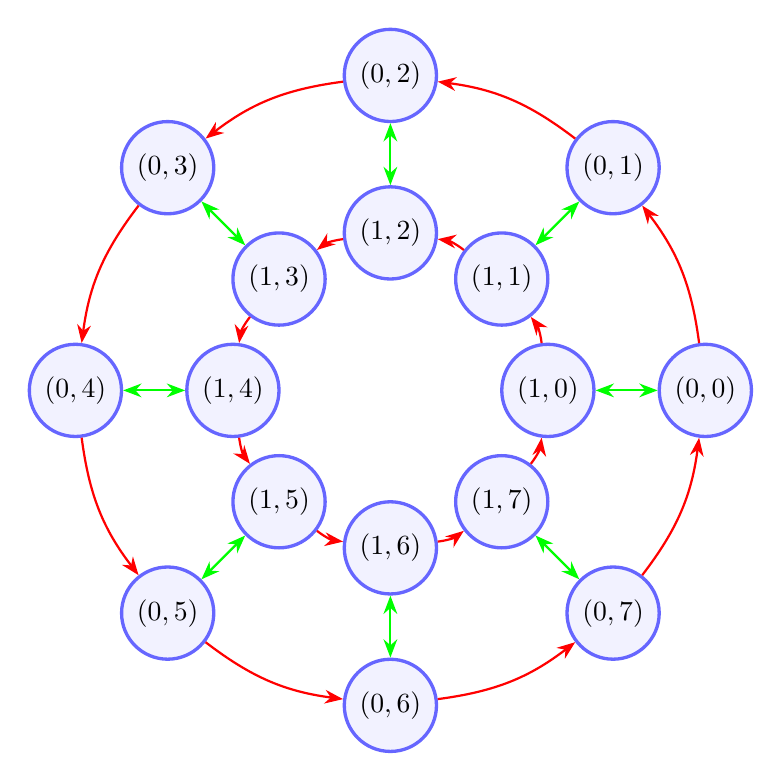
\begin{tikzpicture}[node distance=2cm, 
                            vertex/.style={circle, draw=blue!60, fill=blue!5, very thick, minimum size=5mm},
                            gen_a/.style={->, >=Stealth, thick, red},
                            gen_b/.style={<->, >=Stealth, thick, green}]

            \node[vertex] (v0) at (0:4)   {$(0,0)$};
            \node[vertex] (v1) at (45:4)  {$(0,1)$};
            \node[vertex] (v2) at (90:4)  {$(0,2)$};
            \node[vertex] (v3) at (135:4) {$(0,3)$};
            \node[vertex] (v4) at (180:4) {$(0,4)$};
            \node[vertex] (v5) at (225:4) {$(0,5)$};
            \node[vertex] (v6) at (270:4) {$(0,6)$};
            \node[vertex] (v7) at (315:4) {$(0,7)$};

            \draw[gen_a] (v0) to[bend right=15] (v1);
            \draw[gen_a] (v1) to[bend right=15] (v2);
            \draw[gen_a] (v2) to[bend right=15] (v3);
            \draw[gen_a] (v3) to[bend right=15] (v4);
            \draw[gen_a] (v4) to[bend right=15] (v5);
            \draw[gen_a] (v5) to[bend right=15] (v6);
            \draw[gen_a] (v6) to[bend right=15] (v7);
            \draw[gen_a] (v7) to[bend right=15] (v0);

            \node[vertex] (i0) at (0:2) {$(1,0)$};
            \node[vertex] (i1) at (45:2) {$(1,1)$};
            \node[vertex] (i2) at (90:2) {$(1,2)$};
            \node[vertex] (i3) at (135:2) {$(1,3)$};
            \node[vertex] (i4) at (180:2) {$(1,4)$};
            \node[vertex] (i5) at (225:2) {$(1,5)$};
            \node[vertex] (i6) at (270:2) {$(1,6)$};
            \node[vertex] (i7) at (315:2) {$(1,7)$};

            \draw[gen_a] (i0) to[bend right=15] (i1);
            \draw[gen_b] (i0) to (v0);
            \draw[gen_a] (i1) to[bend right=15] (i2);
            \draw[gen_b] (i1) to (v1);
            \draw[gen_a] (i2) to[bend right=15] (i3);
            \draw[gen_b] (i2) to (v2);
            \draw[gen_a] (i3) to[bend right=15] (i4);
            \draw[gen_b] (i3) to (v3);
            \draw[gen_a] (i4) to[bend right=15] (i5);
            \draw[gen_b] (i4) to (v4);
            \draw[gen_a] (i5) to[bend right=15] (i6);
            \draw[gen_b] (i5) to (v5);
            \draw[gen_a] (i6) to[bend right=15] (i7);
            \draw[gen_b] (i6) to (v6);
            \draw[gen_a] (i7) to[bend right=15] (i0);
            \draw[gen_b] (i7) to (v7);
        \end{tikzpicture}
      \end{figure}

      Las flechas rojas corresponden a operar con el generador $(0, 1)$ y las verdes a operar con 
      $(1, 0)$.
      \newpage

    \subsection{Cuando $a = 3$}
      Vemos que $(0, 1)(0, 1) = (0, 1 + 3^0 1 \mod 8) = (0, 2)$, luego, $(0, 1)^j = (0, j \mod 8)$.

      Ahora, $(0, j)(1, 0) = (1, j + 3^0 0 \mod 8) = (1, j)$.

      Y por último $(1, j)(0, 1) = (1, j + 3^1 1 \mod 8) = (1, j+3 \mod 8)$.

      \begin{figure}[htbp]
        \centering 
        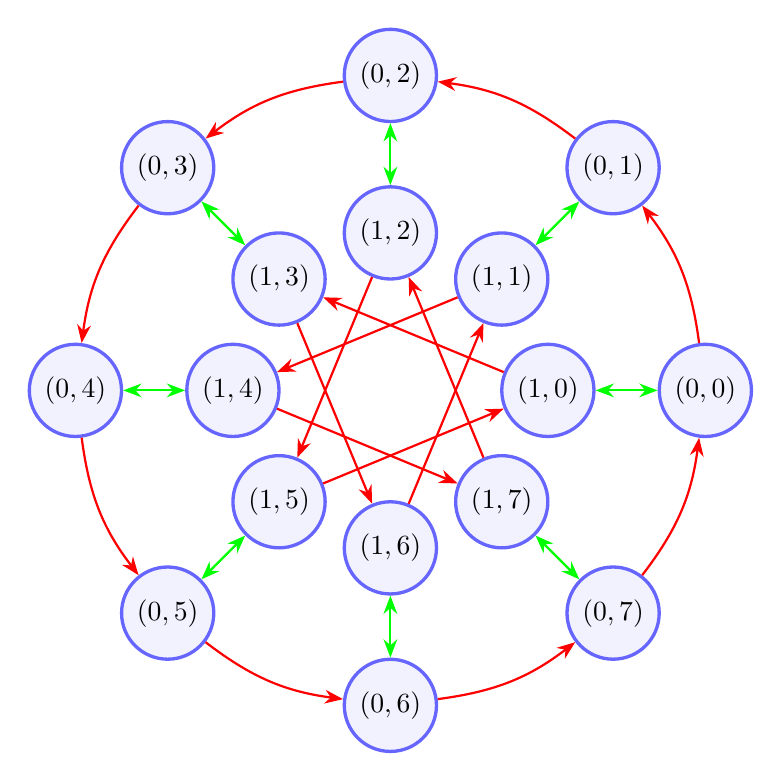
\begin{tikzpicture}[node distance=2cm, 
                            vertex/.style={circle, draw=blue!60, fill=blue!5, very thick, minimum size=5mm},
                            gen_a/.style={->, >=Stealth, thick, red},
                            gen_b/.style={<->, >=Stealth, thick, green}]

            \node[vertex] (v0) at (0:4)   {$(0,0)$};
            \node[vertex] (v1) at (45:4)  {$(0,1)$};
            \node[vertex] (v2) at (90:4)  {$(0,2)$};
            \node[vertex] (v3) at (135:4) {$(0,3)$};
            \node[vertex] (v4) at (180:4) {$(0,4)$};
            \node[vertex] (v5) at (225:4) {$(0,5)$};
            \node[vertex] (v6) at (270:4) {$(0,6)$};
            \node[vertex] (v7) at (315:4) {$(0,7)$};

            \draw[gen_a] (v0) to[bend right=15] (v1);
            \draw[gen_a] (v1) to[bend right=15] (v2);
            \draw[gen_a] (v2) to[bend right=15] (v3);
            \draw[gen_a] (v3) to[bend right=15] (v4);
            \draw[gen_a] (v4) to[bend right=15] (v5);
            \draw[gen_a] (v5) to[bend right=15] (v6);
            \draw[gen_a] (v6) to[bend right=15] (v7);
            \draw[gen_a] (v7) to[bend right=15] (v0);

            \node[vertex] (i0) at (0:2) {$(1,0)$};
            \node[vertex] (i1) at (45:2) {$(1,1)$};
            \node[vertex] (i2) at (90:2) {$(1,2)$};
            \node[vertex] (i3) at (135:2) {$(1,3)$};
            \node[vertex] (i4) at (180:2) {$(1,4)$};
            \node[vertex] (i5) at (225:2) {$(1,5)$};
            \node[vertex] (i6) at (270:2) {$(1,6)$};
            \node[vertex] (i7) at (315:2) {$(1,7)$};

            \draw[gen_b] (i0) to (v0);
            \draw[gen_b] (i1) to (v1);
            \draw[gen_b] (i2) to (v2);
            \draw[gen_b] (i3) to (v3);
            \draw[gen_b] (i4) to (v4);
            \draw[gen_b] (i5) to (v5);
            \draw[gen_b] (i6) to (v6);
            \draw[gen_b] (i7) to (v7);

            \draw[gen_a] (i0) to (i3);
            \draw[gen_a] (i1) to (i4);
            \draw[gen_a] (i2) to (i5);
            \draw[gen_a] (i3) to (i6);
            \draw[gen_a] (i4) to (i7);
            \draw[gen_a] (i5) to (i0);
            \draw[gen_a] (i6) to (i1);
            \draw[gen_a] (i7) to (i2);
        \end{tikzpicture}
      \end{figure}
      \newpage

    \subsection{Cuando $a = 5$}
      Vemos que $(0, 1)(0, 1) = (0, 1 + 5^0 1 \mod 8) = (0, 2)$, luego, $(0, 1)^j = (0, j \mod 8)$.

      Ahora, $(0, j)(1, 0) = (1, j + 5^0 0 \mod 8) = (1, j)$.

      Y por último $(1, j)(0, 1) = (1, j + 5^1 1 \mod 8) = (1, j+5 \mod 8)$.

      \begin{figure}[htbp]
        \centering 
        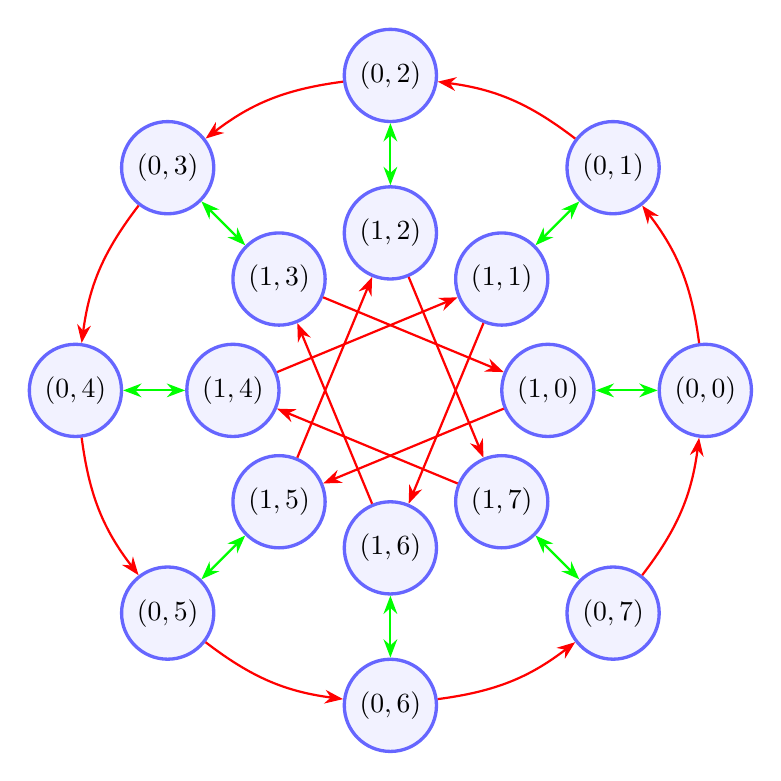
\begin{tikzpicture}[node distance=2cm, 
                            vertex/.style={circle, draw=blue!60, fill=blue!5, very thick, minimum size=5mm},
                            gen_a/.style={->, >=Stealth, thick, red},
                            gen_b/.style={<->, >=Stealth, thick, green}]

            \node[vertex] (v0) at (0:4)   {$(0,0)$};
            \node[vertex] (v1) at (45:4)  {$(0,1)$};
            \node[vertex] (v2) at (90:4)  {$(0,2)$};
            \node[vertex] (v3) at (135:4) {$(0,3)$};
            \node[vertex] (v4) at (180:4) {$(0,4)$};
            \node[vertex] (v5) at (225:4) {$(0,5)$};
            \node[vertex] (v6) at (270:4) {$(0,6)$};
            \node[vertex] (v7) at (315:4) {$(0,7)$};

            \draw[gen_a] (v0) to[bend right=15] (v1);
            \draw[gen_a] (v1) to[bend right=15] (v2);
            \draw[gen_a] (v2) to[bend right=15] (v3);
            \draw[gen_a] (v3) to[bend right=15] (v4);
            \draw[gen_a] (v4) to[bend right=15] (v5);
            \draw[gen_a] (v5) to[bend right=15] (v6);
            \draw[gen_a] (v6) to[bend right=15] (v7);
            \draw[gen_a] (v7) to[bend right=15] (v0);

            \node[vertex] (i0) at (0:2) {$(1,0)$};
            \node[vertex] (i1) at (45:2) {$(1,1)$};
            \node[vertex] (i2) at (90:2) {$(1,2)$};
            \node[vertex] (i3) at (135:2) {$(1,3)$};
            \node[vertex] (i4) at (180:2) {$(1,4)$};
            \node[vertex] (i5) at (225:2) {$(1,5)$};
            \node[vertex] (i6) at (270:2) {$(1,6)$};
            \node[vertex] (i7) at (315:2) {$(1,7)$};

            \draw[gen_b] (i0) to (v0);
            \draw[gen_b] (i1) to (v1);
            \draw[gen_b] (i2) to (v2);
            \draw[gen_b] (i3) to (v3);
            \draw[gen_b] (i4) to (v4);
            \draw[gen_b] (i5) to (v5);
            \draw[gen_b] (i6) to (v6);
            \draw[gen_b] (i7) to (v7);

            \draw[gen_a] (i0) to (i5);
            \draw[gen_a] (i1) to (i6);
            \draw[gen_a] (i2) to (i7);
            \draw[gen_a] (i3) to (i0);
            \draw[gen_a] (i4) to (i1);
            \draw[gen_a] (i5) to (i2);
            \draw[gen_a] (i6) to (i3);
            \draw[gen_a] (i7) to (i4);
        \end{tikzpicture}
      \end{figure}
      \newpage

    \subsection{Cuando $a = 7$}
      Vemos que $(0, 1)(0, 1) = (0, 1 + 7^0 1 \mod 8) = (0, 2)$, luego, $(0, 1)^j = (0, j \mod 8)$.

      Ahora, $(0, j)(1, 0) = (1, j + 7^0 0 \mod 8) = (1, j)$.

      Y por último $(1, j)(0, 1) = (1, j + 7^1 1 \mod 8) = (1, j+7 \mod 8)$.

      \begin{figure}[htbp]
        \centering 
        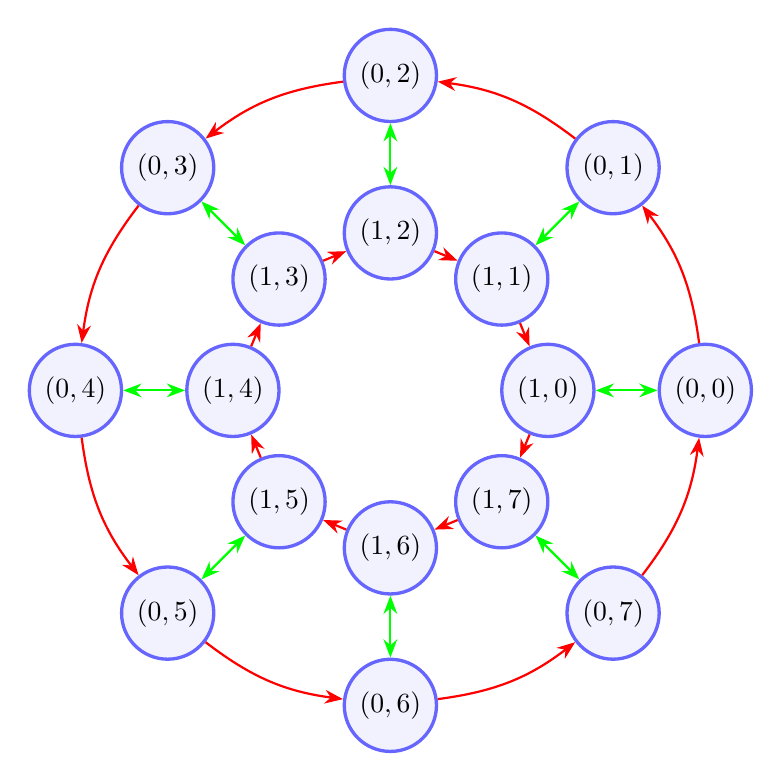
\begin{tikzpicture}[node distance=2cm, 
                            vertex/.style={circle, draw=blue!60, fill=blue!5, very thick, minimum size=5mm},
                            gen_a/.style={->, >=Stealth, thick, red},
                            gen_b/.style={<->, >=Stealth, thick, green}]

            \node[vertex] (v0) at (0:4)   {$(0,0)$};
            \node[vertex] (v1) at (45:4)  {$(0,1)$};
            \node[vertex] (v2) at (90:4)  {$(0,2)$};
            \node[vertex] (v3) at (135:4) {$(0,3)$};
            \node[vertex] (v4) at (180:4) {$(0,4)$};
            \node[vertex] (v5) at (225:4) {$(0,5)$};
            \node[vertex] (v6) at (270:4) {$(0,6)$};
            \node[vertex] (v7) at (315:4) {$(0,7)$};

            \draw[gen_a] (v0) to[bend right=15] (v1);
            \draw[gen_a] (v1) to[bend right=15] (v2);
            \draw[gen_a] (v2) to[bend right=15] (v3);
            \draw[gen_a] (v3) to[bend right=15] (v4);
            \draw[gen_a] (v4) to[bend right=15] (v5);
            \draw[gen_a] (v5) to[bend right=15] (v6);
            \draw[gen_a] (v6) to[bend right=15] (v7);
            \draw[gen_a] (v7) to[bend right=15] (v0);

            \node[vertex] (i0) at (0:2) {$(1,0)$};
            \node[vertex] (i1) at (45:2) {$(1,1)$};
            \node[vertex] (i2) at (90:2) {$(1,2)$};
            \node[vertex] (i3) at (135:2) {$(1,3)$};
            \node[vertex] (i4) at (180:2) {$(1,4)$};
            \node[vertex] (i5) at (225:2) {$(1,5)$};
            \node[vertex] (i6) at (270:2) {$(1,6)$};
            \node[vertex] (i7) at (315:2) {$(1,7)$};

            \draw[gen_b] (i0) to (v0);
            \draw[gen_b] (i1) to (v1);
            \draw[gen_b] (i2) to (v2);
            \draw[gen_b] (i3) to (v3);
            \draw[gen_b] (i4) to (v4);
            \draw[gen_b] (i5) to (v5);
            \draw[gen_b] (i6) to (v6);
            \draw[gen_b] (i7) to (v7);

            \draw[gen_a] (i0) to (i7);
            \draw[gen_a] (i1) to (i0);
            \draw[gen_a] (i2) to (i1);
            \draw[gen_a] (i3) to (i2);
            \draw[gen_a] (i4) to (i3);
            \draw[gen_a] (i5) to (i4);
            \draw[gen_a] (i6) to (i5);
            \draw[gen_a] (i7) to (i6);
        \end{tikzpicture}
      \end{figure}
\end{document}
